\section{Analysis}

Analyzing very large traces can take a long time.  While our custom
binary format enables efficient analysis, and our analysis techniques
are efficient, it can still take 4-8 hours to analyze a single set of
the 2007 traces.  In practice, we analyze the traces in parallel on a
small cluster of 4 core 2.4GhZ Opterons.  Our analysis typically
becomes bottlenecked on the fileservers that serve up to 200MB/s each
once an analysis is running on more than 20 machines.

\subsection{Capture performance}

We start our analysis by looking at the performance of our capture
tool.  We examine the capture rate of the tool by calculating the
megabits/s (Mbps) and kilopackets/s (kpps) for overlapping intervals
of a specified length.  For example if our interval length is 60
seconds, then we will calculate the bandwidth for the interval 0s-60s,
3s-63s, 6s-66s, ... end-of-trace.  We chose to calculate the bandwidth
for overlapping intervals so that if there is any aligned cyclicality
in the trace data we will not be confused by it.  We divide an
interval into 20 sub-intervals.  We then take the data and put it into
an approximate quantile so that we can understand the distribution of
rates even for small intervals.  For example, we have 11.6 bilion
measurements for nfs-2/set-0 at a 1ms interval length.  This
corresponsd to the 6.7 days of that trace.
% 11.6 * 10^9 * 0.001 / 20 = 580,000 / 86400 = 6.7

Figure~\ref{fig:mbps-nfs-2} shows the cdf of bandwidth for the 2007
traces using 60 second intervals.  Two traces stand out set-5 and
set-4.  Set-4 was a trace of an NFS cache, rather than clients, and so
shows a much lower aggregate rate.  Set-5 was the trace of a different
set of clients working on a different movie, and hence shows a very
different distribution.  The graph shows the effectiveness of our
tracing technology on real workloads as it can capture 60s intervals
above 3Gbits (375MB/s).  Indeed these traces show the requirement for
high speed tracing as 5-20\% of the traces intervals have sustained
intervals above 1Gbit, which is above the rate at which
Leung~\cite{LeungUsenix08} noted their tracing tool started to drop
packets.  The 2003 traces in figure~\ref{fig:mbps-nfs-1} show a wider
distribution of shapes because they were taken on a wider variety of
places in the network.  The rates are also much lower because our 2003
capture technology could not capture as much data, so we traced fewer
machines at a time.

Figure~\ref{fig:nfs-2-set-5-intervals} shows nfs-2/set-5 at different
interval lengths.  This graph emphasizes how bursty the traffic was
during this trace. While 50\% of the intervals were above 500Mbits for
60s intervals, only 30\% of the intervals were above 500Mbits for 1ms
intervals.

Figure~\ref{fig:capture-tails} shows the tail of the distributions for
the capture rates for two of the trace sets.  The relative similarity
between the Mbps and kpps graphs is simply because packet size
distributions are relatively constant.  The nfs-1 trace lines are
distorted by the fact that in these regions we expect the 2003 capture
tool was dropping packets.  The traces show the remarkably high
burstiness of the 2007 traces.  While 90\% of the 1ms intervals are
below 2Gbits, 0.1\% are above 6Gbits.  We expect we would have seen
slightly higher rates, but because of our configuration error for the
2007 capture tool, we could not capture above about 8Gbits.

\begin{figure}
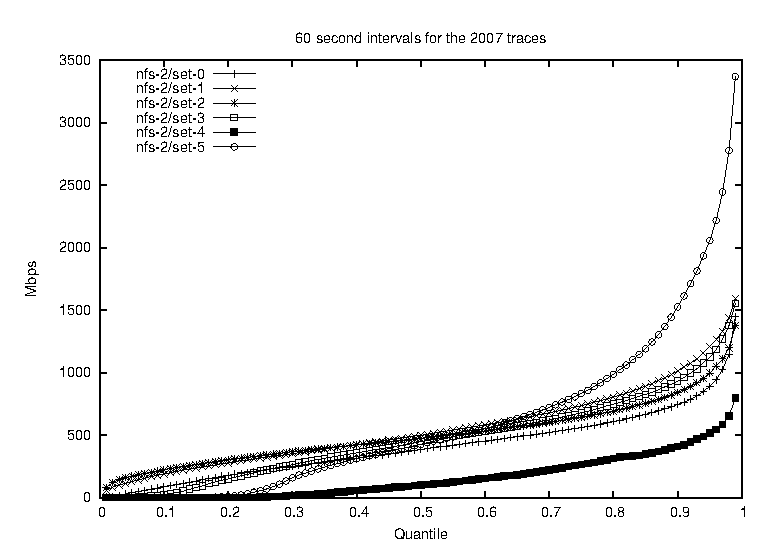
\epsfig{width=3.2in, angle=0, file=graphs/Mbps-nfs-2.ps}
\caption{...}
\label{fig:mbps-nfs-2}
\end{figure}

\begin{figure}
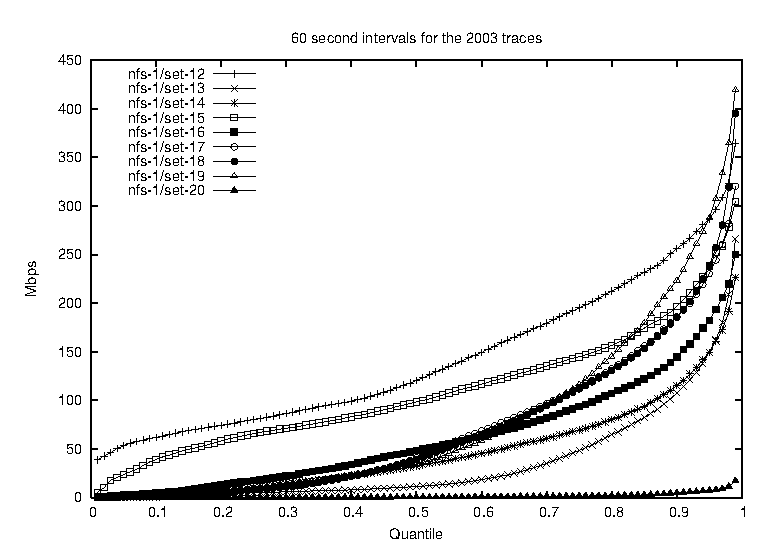
\epsfig{width=3.2in, angle=0, file=graphs/Mbps-nfs-1.ps}
\caption{...}
\label{fig:mbps-nfs-1}
\end{figure}

\begin{figure}
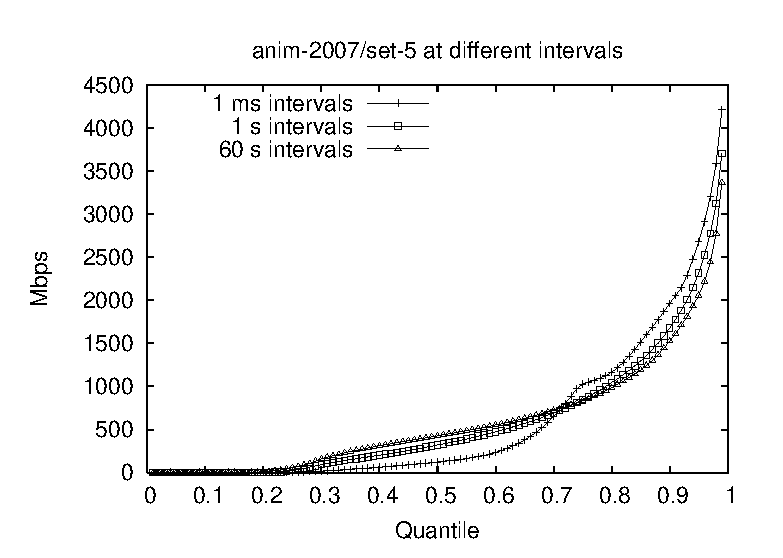
\epsfig{width=3.2in, angle=0, file=graphs/Mbps-nfs-2-set-5.ps}
\caption{...}
\label{fig:nfs-2-set-5-intervals}
\end{figure}

\begin{figure}
\epsfig{width=3.2in, angle=0, file=graphs/Mbps-tails.ps}
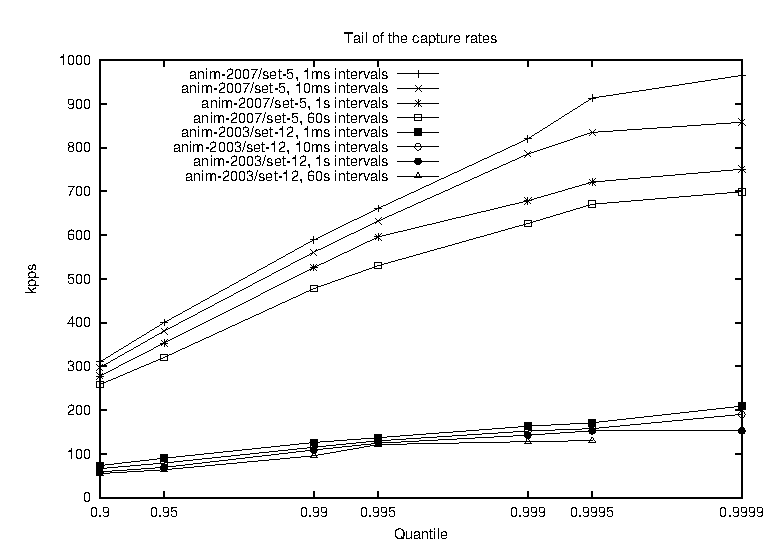
\epsfig{width=3.2in, angle=0, file=graphs/kpps-tails.ps}
\caption{...}
\label{fig:capture-tails}
\end{figure}

\subsection{Basic NFS analysis}

% nfs_hostinfo_rates, nfs_hostinfo_rate_quantiles, nfs_hostinfo_cube;
% choose sets nfs-2/set-[2,5]; nfs-1/set-[5,12]
%                     03+10, 06+13 ; 20+42, 27+49

% select from_unixtime(group_time), group_count/3600 where dataset = 'nfs-1/set-12' and group_time is not null and host is null  and operation is null and direction is null and op_dir is null
% nfs-1/set-5: 2003-09-16 .. 2003-09-18
% nfs-1/set-12: 2003-12-09 - 2003-12-10
% nfs-2/set-2: 2007-03-05 .. 2007-03-11
% nfs-2/set-5: 2007-10-12 .. 2007-10-17
% from hostinfo.hg + a few minor tweaks (n/a) for set-5 readdirplus
\begin{table*}
\begin{tabular}{|r||r|r||r|r||r|r||r|r|}
\hline
  & \multicolumn{2}{c||}{nfs-1/set-12} & \multicolumn{2}{c||}{nfs-1/set-5} & \multicolumn{2}{c||}{nfs-2/set-2} & \multicolumn{2}{c|}{nfs-2/set-5} \\
   operation &   Mops & bytes/op &   Mops & bytes/op &   Mops & bytes/op &   Mops & bytes/op \\
\hline
     symlink &     0.008 &   201 &     0.000 &    92 &     0.001 &   415 &     0.000 &   458 \\
       rmdir &     0.204 &   152 &     0.001 &    64 &     0.020 &   167 &     0.002 &   178 \\
       mkdir &     0.173 &   304 &     0.005 &   193 &     0.071 &   336 &     0.004 &   334 \\
      rename &     0.028 &   270 &     0.002 &   150 &     0.250 &   367 &     0.055 &   348 \\
\hline
      fsinfo &     0.023 &   176 &     0.003 &    72 &     1.352 &   176 &     0.619 &   176 \\
        link &     0.000 &    86 &     0.000 &    88 &     3.259 &   314 &     0.182 &   322 \\
        null &     0.259 &     5 &     0.087 &     4 &     1.482 &     4 &     2.808 &     4 \\
      create &     0.296 &   295 &     0.965 &   200 &     4.639 &   367 &     1.616 &   344 \\
\hline
      remove &     0.275 &   136 &     0.641 &    69 &     8.419 &   194 &     1.500 &   186 \\
     setattr &     0.716 &   133 &     1.075 &   136 &     9.415 &   193 &     6.531 &   192 \\
     readdir &     4.579 &   281 &     1.132 &  3940 &    28.318 &  4089 &    18.350 &  4071 \\
 readdirplus &     0.632 &  2307 &     0.000 &  n/a  &    32.806 &  1890 &    20.271 &  2001 \\
\hline
    readlink &     0.081 &    74 &     0.049 &    79 &    25.421 &   204 &    42.335 &   203 \\
      fsstat &    19.875 &    56 &    50.416 &    56 &     0.017 &   180 &     0.003 &   180 \\
       write &    14.546 &  9637 &    30.236 &  7880 &    32.390 & 13562 &    45.177 & 15015 \\
      lookup &   134.108 &    83 &    82.823 &    92 &   643.854 &   239 &   807.127 &   235 \\
\hline
        read &   345.743 &  1231 &   165.969 &  7855 &  1460.669 & 14658 &  1761.199 & 12301 \\
      access &     1.858 &   136 &     0.000 &   136 &  4000.204 &   136 &  3570.404 &   136 \\
     getattr &   244.650 &   104 &   967.961 &   104 &  6598.515 &   124 &  2756.785 &   123 \\
\hline
 {\bf total} &   768.053 &   790 &  1301.364 &  1274 & 12851.102 &  1833 &  9034.968 &  2599 \\
\hline
\end{tabular}
\caption{...}
\label{table:nfs-stats-overview}
\end{table*}

Table~\ref{table:nfs-stats-overview} provides an overview of all the
operations that occurred in the four traces we are examining in more
detail.  It shows a number of substantial changes in the workload
presented to the NFS subsystem.  First, the read and write sizes have
almost doubled from the nfs-1 to nfs-2 datasets.  This is expected
because the customer moved from nfs-v2 to nfs-v3 between the two
tracing periods, and set the v3 read/write size to 16k.  We asked and
were told they set it to those sized based on some performance
measurements of sequential I/O.  The NFS version switch also accounts
for the increase in access calls (new in V3), and readdirplus (also
new in V3).  

We also see that this workload is incredibly read-heavy.  This is
expected; the animation workload does reads a very large amount of
textures, models, etc to produce a relatively small output frame.
However, we believe that our traces under-estimate the number of write
operations.  We discuss this problem below in the discussion around
operations.  The abnormally low read size for set-12 occurred because
that filer was handling a large number of stale FH requests.  The
replies were therefore small and pulled down the bytes/operation.  We
see a lot more getattr operations in set-5 than set-12 because set-12
is a filer behind some nfs-caches, whereas set-5 is the workload
before the nfs-caches.

Figure~\ref{table:99quant-differences} and
figure~\ref{fig:allops-quantile} shows how long averaging intervals
can distort the load placed on the storage system.  If we were to
develop a storage system for the hourly loads reported in most papers,
we would fail to support the substantially higher near peak (99\%)
loads seen in the data.  It also hides the periods of more idleness
that could be used for incremental scrubbing and data reorganization.

% select dataset, group_seconds, operations_per_second from xnfs_hostinfo_rate_quantiles where host is null and direction = 'send' and operation is null and op_dir is null and quantile = 0.99
\begin{table}
\begin{tabular}{|r|r|r|r|}
\hline
dataset & 1s ops/s & 3600s ops/s & ratio \\
\hline
nfs-1/set-5  & 26445  & 15110 & 1.75x \\
nfs-1/set-12 & 44926 & 19923 & 2.25x \\
nfs-2/set-2  & 75457 & 54657 & 1.38x \\
nfs-2/set-5  & 59726.5 & 41550 & 1.44x \\
\hline
\end{tabular}
\caption{...}
\label{table:99quant-differences}
\end{table}

\begin{figure}
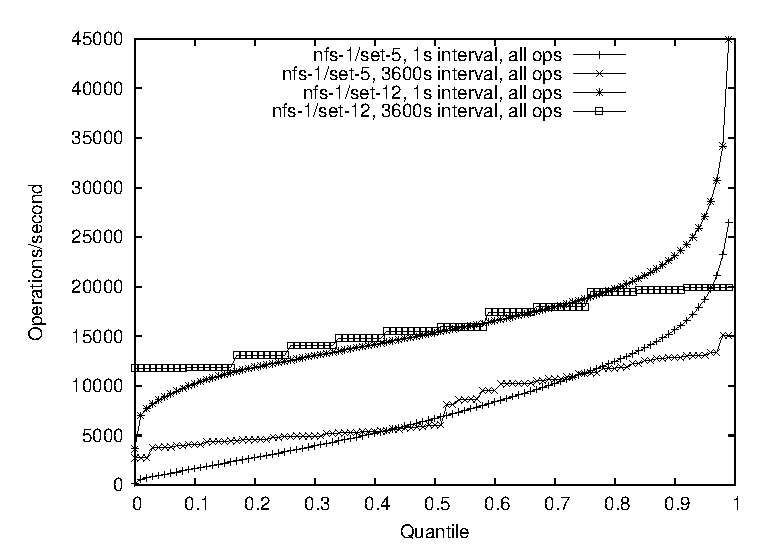
\epsfig{width=3.2in, angle=0, file=graphs/allops-quantile-nfs-1.ps}
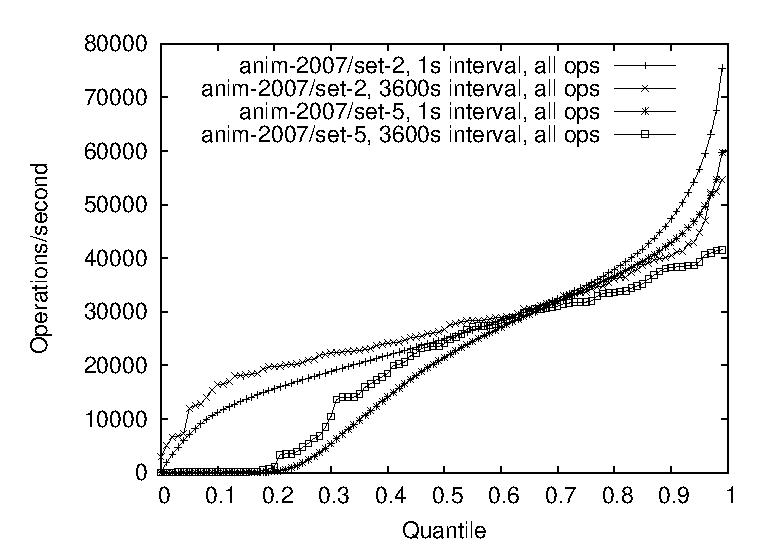
\epsfig{width=3.2in, angle=0, file=graphs/allops-quantile-nfs-2.ps}
\caption{...}
\label{fig:allops-quantile}
\end{table}

\begin{figure}
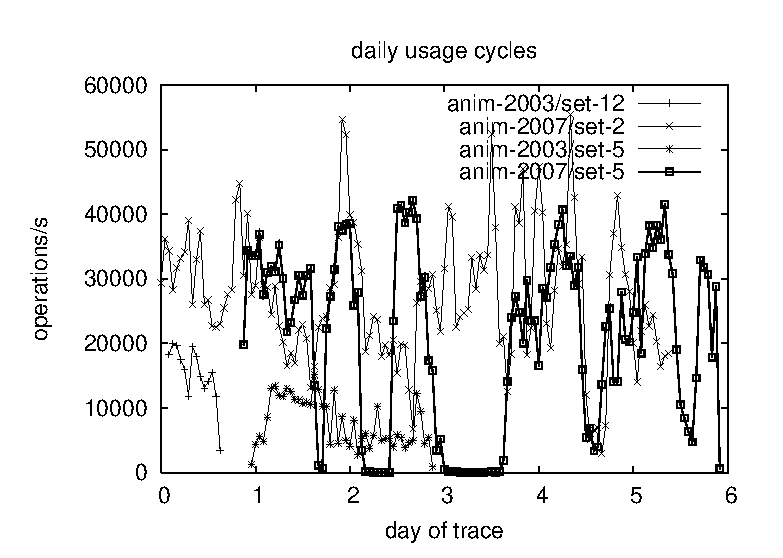
\epsfig{width=3.2in, angle=0, file=graphs/daily-oprate.ps}
\caption{...}
\label{fig:daily-oprate}
\end{figure}

\subsection{Sequentiality}

% select dataset,operation, max(mean_operations_per_second) from xnfs_hostinfo_rates where group_seconds = 1 and host is null and direction = 'send' and operation is not null and op_dir is null and mean_operations_per_second > 300 group by dataset,operation order by operation
% --> access, fsstat, getattr, lookup, read, write 

\begin{figure}
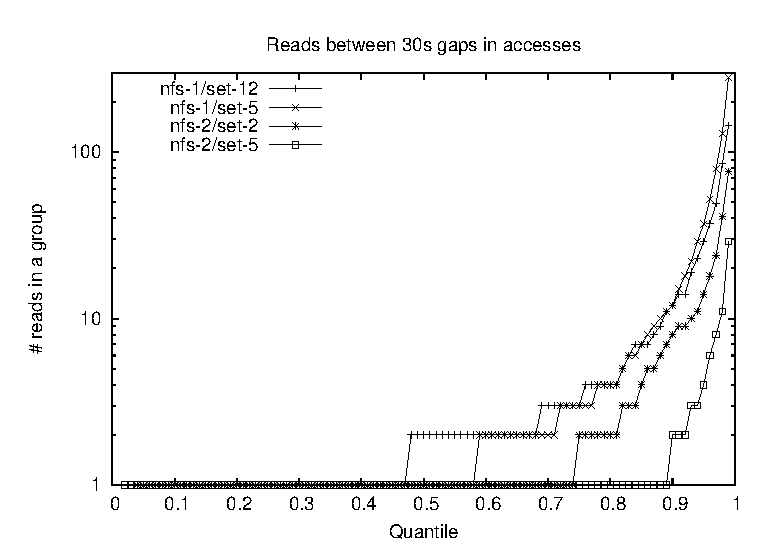
\epsfig{width=3.2in, angle=0, file=graphs/seq-read-group-counts.ps}
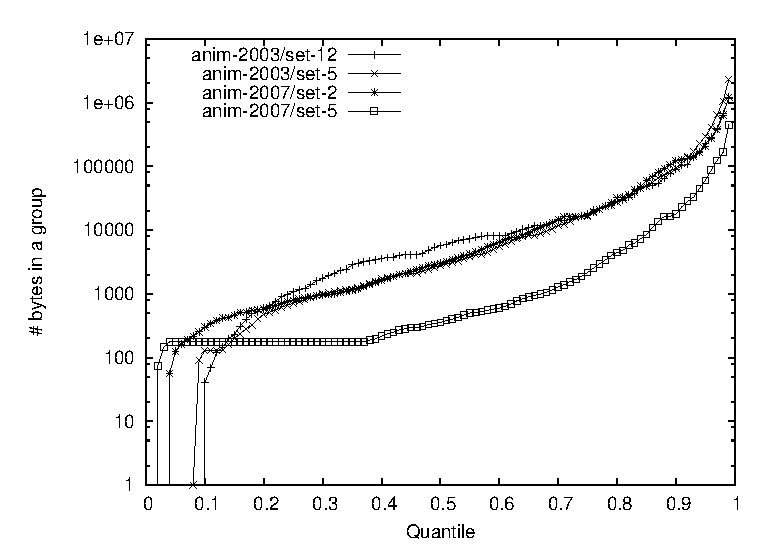
\epsfig{width=3.2in, angle=0, file=graphs/seq-read-group-bytes.ps}
\caption{...}
\label{fig:seq-read-group}
\end{figure}

\begin{figure}
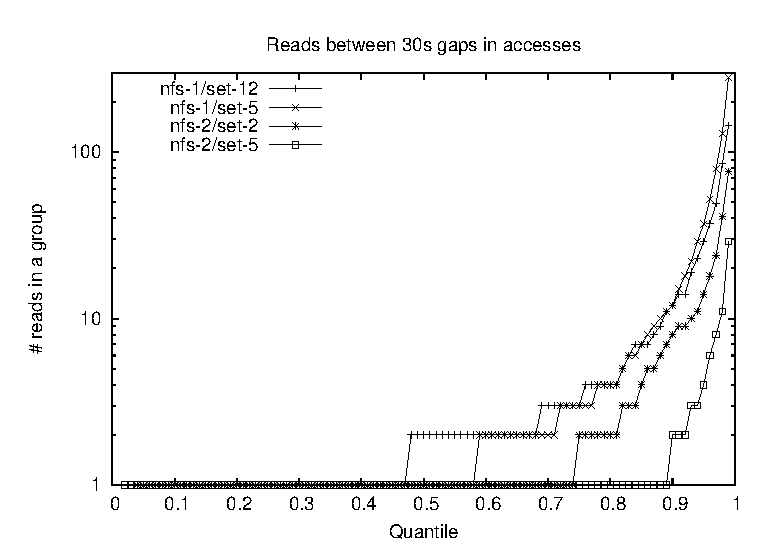
\epsfig{width=3.2in, angle=0, file=graphs/seq-read-group-counts.ps}
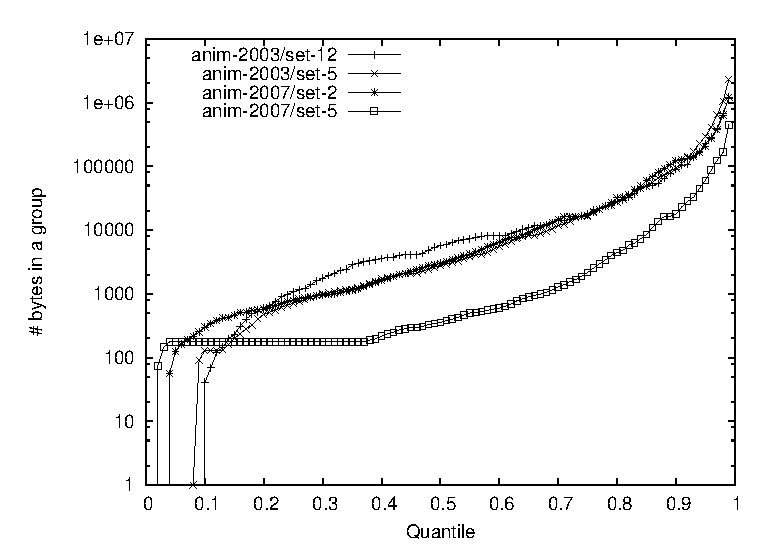
\epsfig{width=3.2in, angle=0, file=graphs/seq-read-group-bytes.ps}
\caption{...}
\label{fig:seq-in-random}
\end{figure}

\begin{figure}
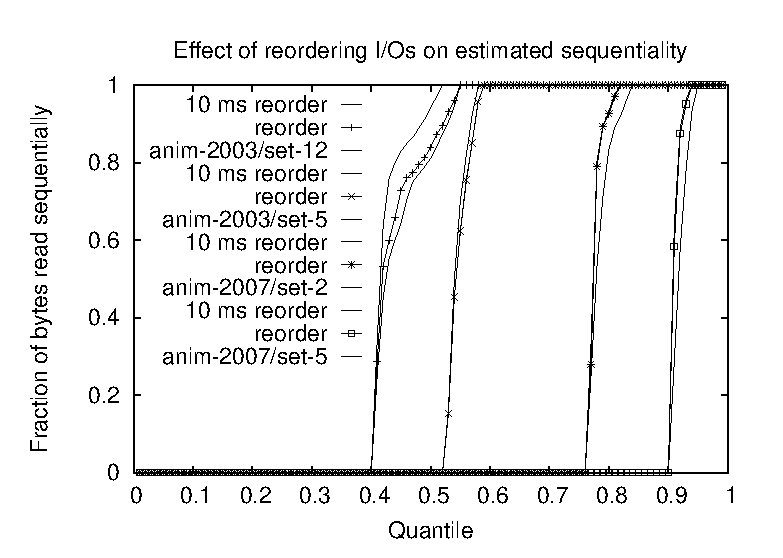
\epsfig{width=3.2in, angle=0, file=graphs/seq-bytes-compare.ps}
\caption{...}
\label{fig:seq-bytes-compare}
\end{figure}
